\chapter{Diseño de paquetes} \label{cap:diseño-paquetes}


\section{Introducción}


% Este capítulo muestra cómo se agrupan por cercanía funcional y semántica las clases y demás elementos del sistema en diferentes paquetes, que permiten su manipulación en grupos. Se identificarán los paquetes más
% relevantes del sistema y se describirá su finalidad.

 \section{Especificación de los paquetes de la aplicación}

% Los paquetes en los que se puede descomponer el simulador se obtienen a partir de los subsistemas que lo constituyen:
% \begin{itemize}
%  \item \textbf{Paquete es.uco.simAS}.
%  \item \textbf{Paquete editor}.
%  \item \textbf{Paquete simulador}.
%  \item \textbf{Paquete util.gramatica}.
%  \item \textbf{Paquete centroayuda}.
%  \item \textbf{Paquete resources}.
% \end{itemize}

% \subsection{Paquete es.uco.simAS}

% Este es el paquete general de la aplicación y contiene a los demás paquetes. Al ser un proyecto de la \textit{Universidad de Córdoba}, se ha seguido la recomendaciones de Java a la hora de nombrar los paquetes y se ha supuesto el dominio \textbf{es.uco.simAS} para nombrar este paquete.

% \subsection{Paquete editor}

% El paquete \textbf{editor} contiene todas las clases del editor de gramáticas (tanto las de información como las que solamente contienen elementos gráficos). El paquete importa a los paquetes \textit{util.gramatica}, para hacer uso de las gramáticas de contexto libre; \textit{centroayuda}, para interactuar con la ayuda; \textit{resources}, donde se almacenan todos los iconos y recursos gráficos para la interfaz; y el \textit{paquete del simulador}, lo importa para poder transferirle una gramática (Figura  \ref{paqeditor}).

% \begin{figure}[H]
%       \begin{center} 
% 	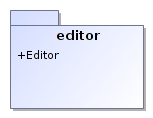
\includegraphics[scale=0.6]{figuras/Cap8/paqeditor.jpg}
% 	\caption{Paquete editor}
% 	\label{paqeditor}
%       \end{center}
%   \end{figure}


% \subsection{Paquete simulador}

% El paquete \textbf{simulador} contiene todas las clases del simulador de gramáticas (tanto las de información como las que solamente contienen elementos gráficos). El paquete importa a los paquetes \textit{util.gramatica}, para hacer uso de las gramáticas de contexto
% libre; \textit{centroayuda}, para interactuar con la ayuda; \textit{resources}, donde se almacenan todos los iconos y recursos gráficos para la interfaz; y el \textit{paquete del editor} lo  importa para poder transferirle una gramática de vuelta (Figura  \ref{paqsimulador}).

% \begin{figure}[H]
%       \begin{center} 
% 	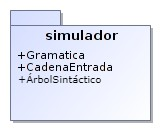
\includegraphics[scale=0.6]{figuras/Cap8/paqsimulador.jpg}
% 	\caption{Paquete simulador}
% 	\label{paqsimulador}
%       \end{center}
%   \end{figure}

% \subsection{Paquete util.gramatica}

% Este paquete contiene todas las clases relacionadas con las gramáticas de contexto libre, además de la clase que representa a las funciones de error (Figura \ref{paqgramatica}).

% \begin{figure}[H]
%       \begin{center} 
% 	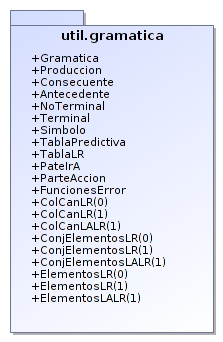
\includegraphics[scale=0.6]{figuras/Cap8/paqgramatica.jpg}
% 	\caption{Paquete util.gramatica}
% 	\label{paqgramatica}
%       \end{center}
%   \end{figure}

% \subsection{Paquete centroayuda}

% Este paquete contiene la ventana del centro de ayuda y todos los recursos de la ayuda de SimAS (todos los capítulos en formato html de la ayuda) (Figura \ref{paqayuda}=.

% \begin{figure}[H]
%       \begin{center} 
% 	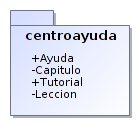
\includegraphics[scale=0.6]{figuras/Cap8/paqayuda.jpg}
% 	\caption{Paquete centroayuda}
% 	\label{paqayuda}
%       \end{center}
%   \end{figure}

% \subsection{Paquete resources}

% Este paquete contiene todos los recursos gráficos utilizados por los componentes de la interfaz gráfica de SimAS (iconos, imágenes, tipos de letra, etcétera). Nótese que los componentes de la ayuda se han situado en el paquete \textit{centroayuda} en lugar de hacerlo en este. Así se asegura que todos los recursos gráficos usados por el programa están en el mismo paquete y separados de otros recursos que sólo usa un módulo concreto, como es el Centro de ayuda.

% Este paquete aparece vacío en el diagrama porque realmente no contiene
% ninguna clase de las especificadas en el estudio del sistema, sino que contiene recursos gráficos de la interfaz (que son demasiados como para enumerarlos en el diagrama).

 \section{Diagrama de paquetes de la aplicación}

% En la figura \ref{dpaquetes} se muestra el diagrama de paquetes del simulador, según lo analizado anteriormente. Nótese que en los paquetes únicamente se muestran los elementos de información finales de la aplicación (las clases que representan objetos de la interfaz no se recogen en este diagrama, puesto que complicarían en gran medida
% su presentación y comprensión). 

%  \begin{figure}[H]
%       \begin{center} 
% 	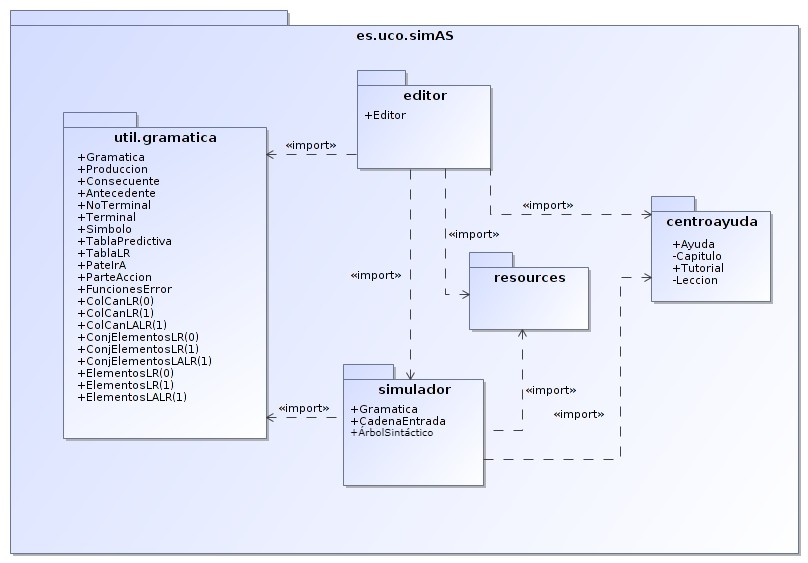
\includegraphics[scale=0.55]{figuras/Cap8/paquetes.jpg}
% 	\caption{Diagrama de paquetes}
% 	\label{dpaquetes}
%       \end{center}
%   \end{figure}


